% !TEX root =  ../geospatial-video.tex

\section{Data Model}
\label{section:data-model}

To interface with the data, the user uses the \textit{Annotation}, \textit{Instance}, \textit{Frame}, and \textit{Video} abstractions.
\begin{itemize}
    \item 
    \textbf{\textit{Video}} represents a video file.
    \item 
    \textbf{\textit{Frame}} represents a video frame in a video file.
    \item 
    \textbf{\textit{Instance}} represents an object that presents in a video. An \emph{Instance} can be present on a video spanning over multiple frames as shown in Figure~\ref{fig:abstraction}.
    \item 
    \textbf{\textit{Annotation}} represents properties of an \emph{Instance} for a specific \emph{Frame}.
\end{itemize}
Figure \ref{fig:abstraction} illustrates this data model in greater detail.
Each video is denoted by an unique scene ID, and frames are indexed by the order in which they appear.
All instances have an unique instance token which can be used to query specific properties for that instance specifically.
By passing the scene ID, the user can load the video with corresponding annotations and properties needed for downstream tasks.
The user may also directly instantiate any Frame and Instance directly from the nuScenes database, if provided with the frame order and instance token in addition to the scene ID.
All metadata are stored in Annotations, with the exception of ``Category" (e.g. ``car", ``person"), which is an attribute in \textit{Instance}.

\newcommand{\dataModelCaption}{
The wealth of image, annotation, spatial, and temporal information in geospatial data is simplified into in our language into Video, Frame, Instance, and Annotation.
A video consists of several consecutive frame, which point to a specific image, and instances (e.g., cars, pedestrians) may persist through many frames.
Each instance contains a category attribute, and an annotations attribute for accessing more detailed metadata of interest.
}

\begin{figure*}[ht]
    \centering
    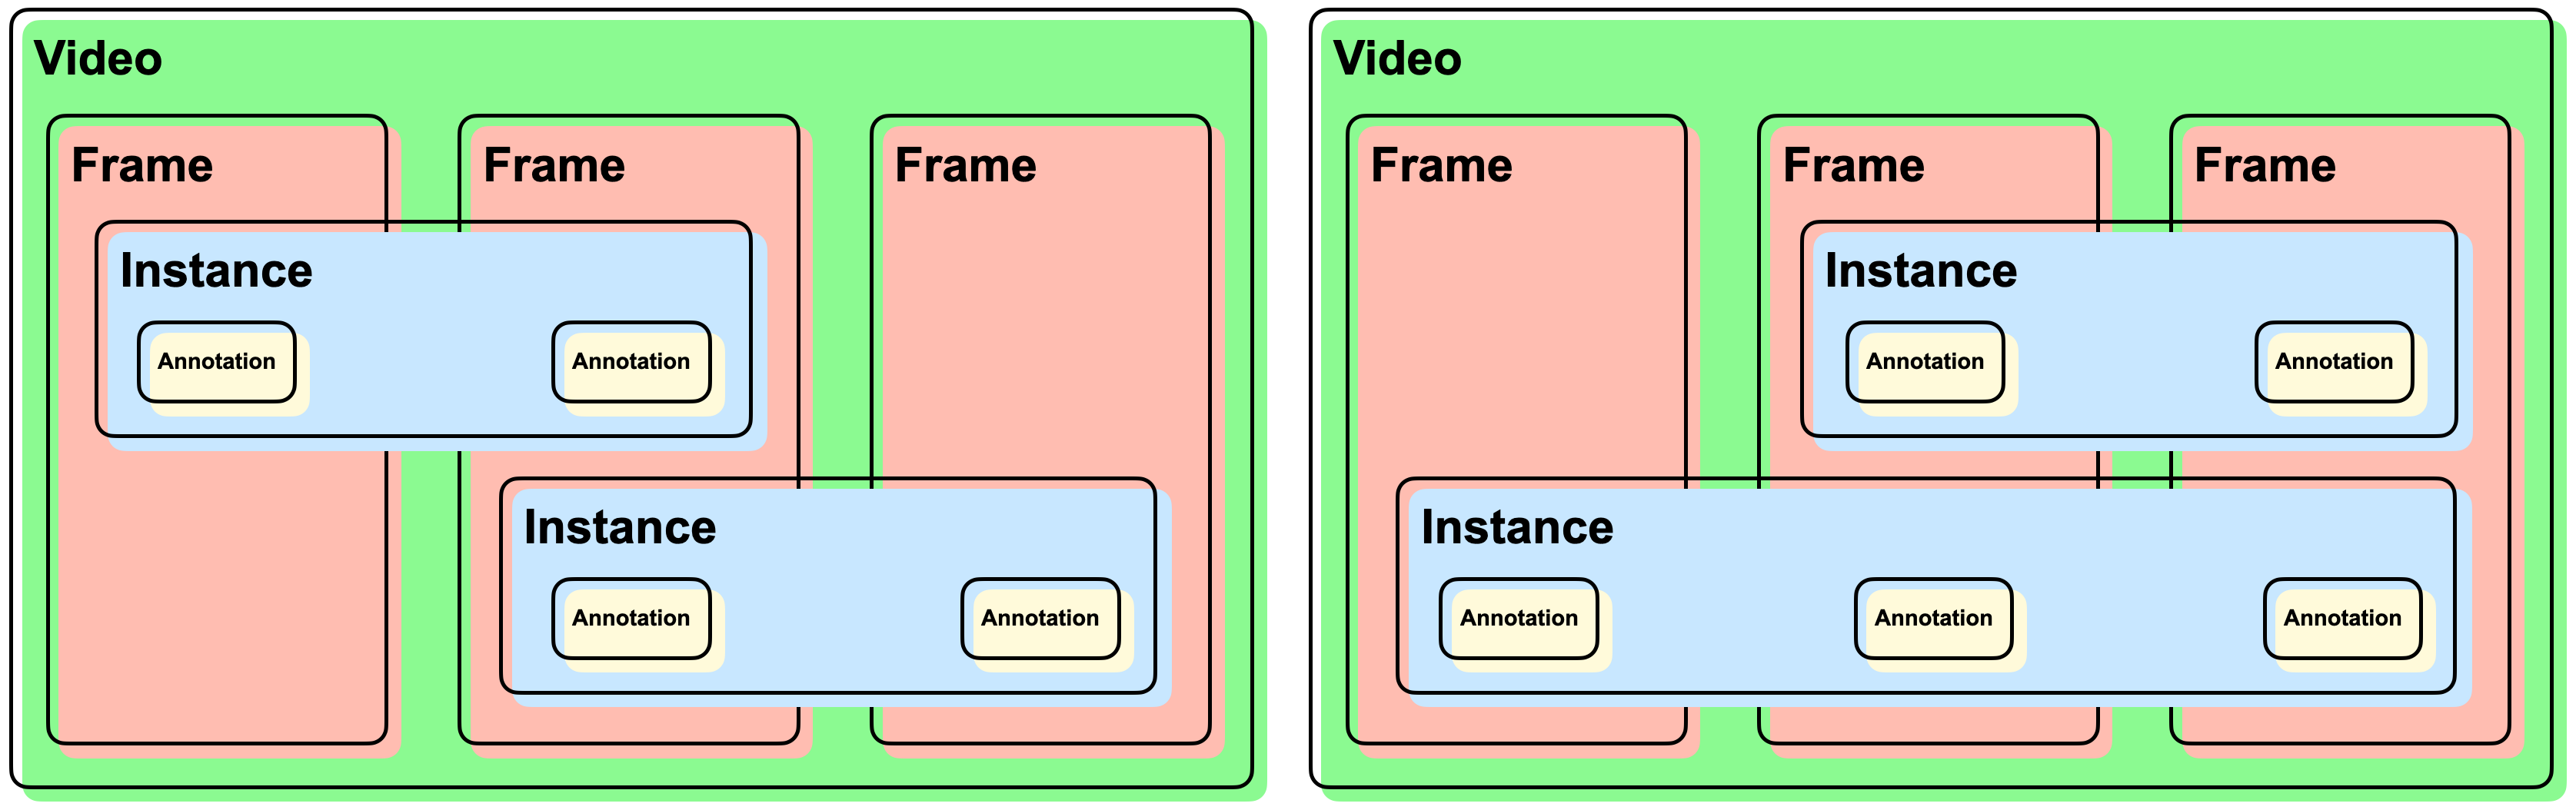
\includegraphics[width=\textwidth]{figures/data-abstraction.png}
    \caption{\dataModelCaption}
    \label{fig:abstraction}
\end{figure*}

\newcommand{\dataHierarchyCaption}{
The hierarchy of our data type.
Users can start exploring they geospatial-video data from \emph{Videos}.
Then, they can choose to explore the data through either \emph{Frames} or \emph{Instances}.
And from both \emph{Frames} and \emph{Instances}, they can explore further to \emph{Annotations}.
In addition, the users have the flexibility in switching between exploring \emph{Frames} and \emph{Instances}.
}

\begin{figure}[ht]
    \centering
    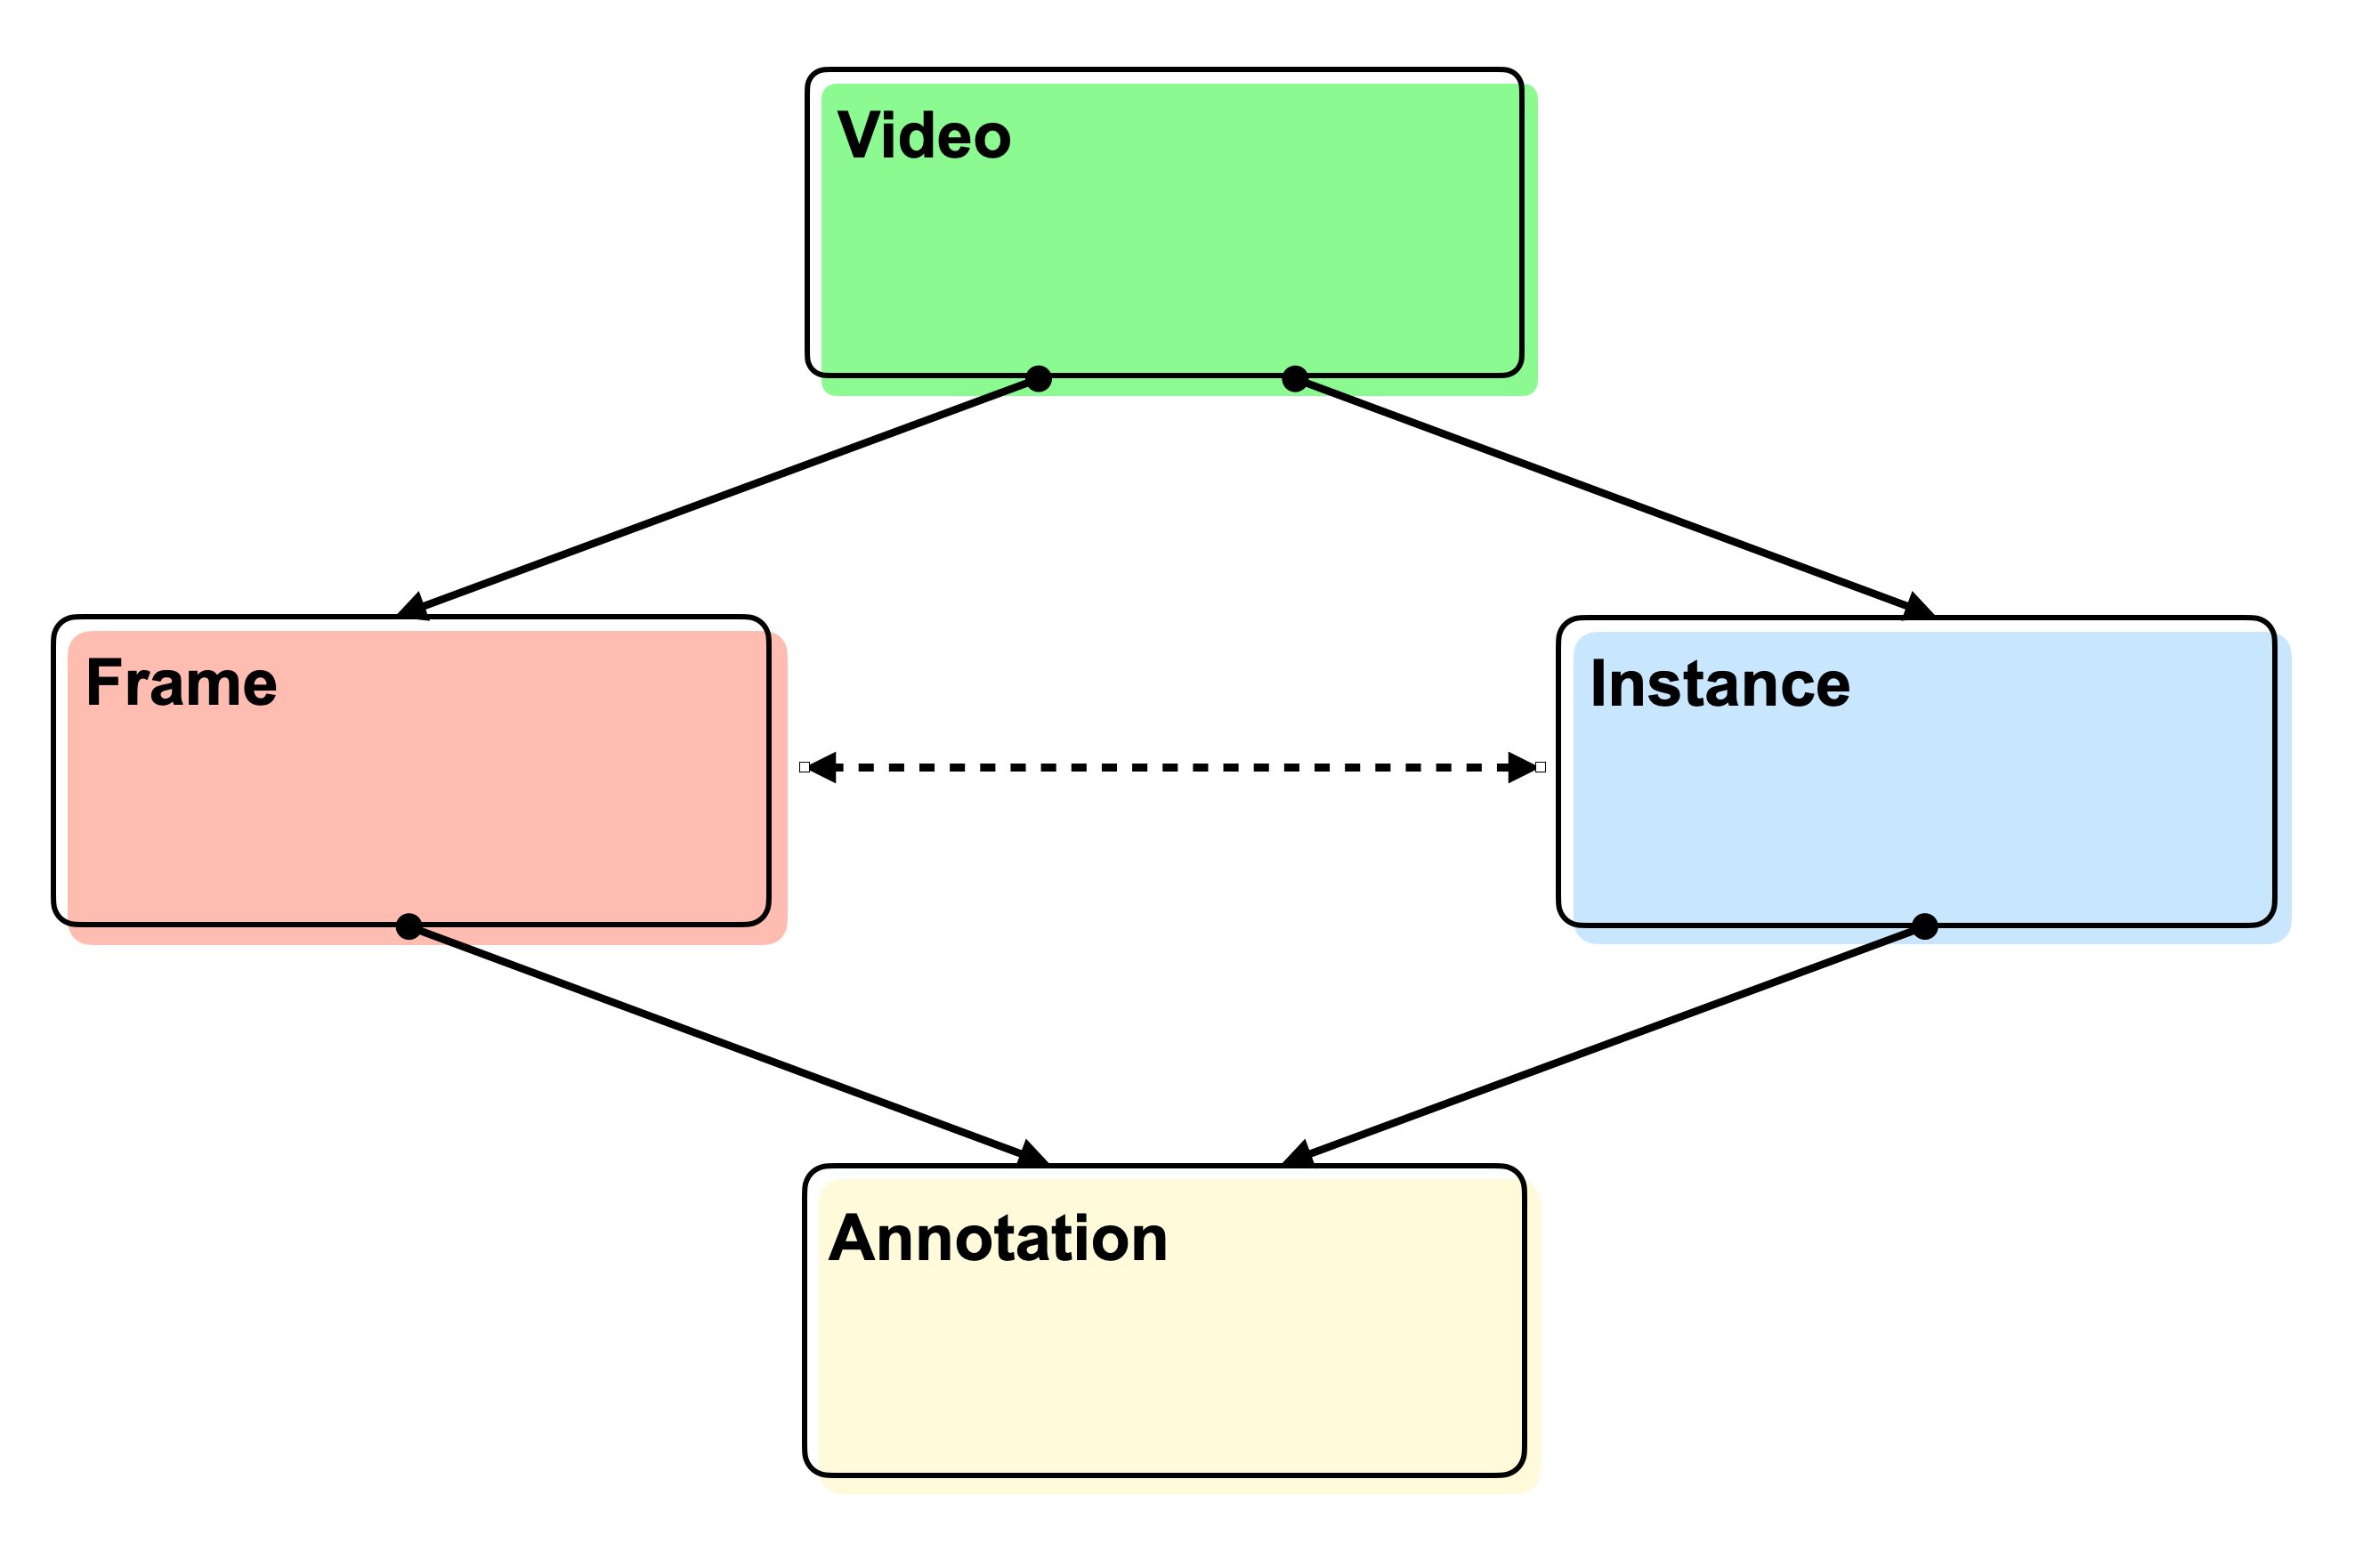
\includegraphics[width=\columnwidth]{figures/data-hierarchy.png}
    \caption{\dataHierarchyCaption}
    \label{fig:hierarchy}
\end{figure}

Our data model is an improvement to Apperception's data model.
In Apperception, users mostly interact with \emph{World}, \emph{Video}, and \emph{Instance}, and do not have access to individual frames of the video.
The output from Apperception can also only represent \emph{World} and \emph{Instance}.
In the new data model, users can interact with all of the data types shown in Figure~\ref{fig:hierarchy}.
This abstraction allows users to construct queries to answer more complex data exploration questions,
while not exposing the internal geospatial data store.
